%-------------------------------------------------------------------------------
\subsubsection{Système proie prédateur} 
%-------------------------------------------------------------------------------

On considère le système proie-prédateur suivant
\begin{equation} \label{eq:L3bioProiePredateur}
\left\{\begin{array}{rcl}
        \dot x & = & \displaystyle{x \left(1 - \frac{x}2\right) - \frac{xy}{1+x}} \\
        \dot y & = & \displaystyle{\frac{x-1}{x+1} y}
       \end{array}\right..
\end{equation}
% dans laquelle $x$ désigne la concentration d'un métabolite : \eqref{eq:L3BioSUTD2E2} modélisant l'ensemble des réactions biochimiques impliquées dans la production/dégradation de ce métabolite.

\begin{enumerate}
\item Qui sont les proies, qui sont les prédateurs ?
  \solution{$x =$ proies, $y = $ prédateurs : 
    \begin{itemize}
    \item Le terme d'interaction $xy$ intervient avec un signe négatif dans le taux de croissance $\dot x$, ce qui est caratéristique du comportement d'une population de proies confrontées à des prédateurs.
    \item Pour $x=0$, on obtient $\dot y = -y$ qui décrit un comportement d'une population de prédateurs qui s'éteint en l'absence de proie. 
    \end{itemize}}
\item Déterminer les points stationnaires du systèmes.
  \solution{En distinguant les cas $y = 0$ et $y \neq 0$, on vérifie facilement que
  $$
  m^*_1 = \left(\begin{array}{c}0 \\ 0\end{array}\right), \qquad
  m^*_2 = \left(\begin{array}{c}2 \\ 0\end{array}\right), \qquad
  m^*_3 = \left(\begin{array}{c}1 \\ 1\end{array}\right)
  $$
  sont les seuls points stationnaires.}
\item Montrer que $y=0$ est une solution du système. Quel est le comportement de $x$ dans ce cas ?
  \solution{$y \equiv 0$ satisfait la seconde équation du système. La première équation devient alors $\dot x = x \left(1 - x/2\right)$ : la population des proies évolue selon un modèle logistique.}
\item Déterminer la matrice jacobienne $J_{x, y}$ du système
  \solution{On a
  $$
  J_{x, y} = \left[\begin{array}{ccc}
                   \displaystyle{(1 - x) - \frac{y}{(1+x)^2}} & & 
                   \displaystyle{\frac{-x}{1+x}} \\
                   \displaystyle{\frac{2 y}{(x+1)^2}} & & 
                   \displaystyle{\frac{x-1}{x+1}}
                  \end{array}\right]
  $$}
  \item \'Etudier la stabilité des points stationnaires.
  \solution{
  \begin{description}
  \item[$m^*_1 = (0, 0) : $] on a 
    $$
    J_{m^*_1} = \left[\begin{array}{ccc}
                    {1} & & 
                    {0} \\
                    {0} & & 
                    {-1/2}
                    \end{array}\right]
    $$
    dont les valeurs propres sont 1 (associée à $u = (1, 0)$) et $-1/2$ (associée à $u = (0, 1)$). \\
    Il s'agit donc d'un point selle : l'équilibre est instable. Plus précisément, il est instable dans la direction de l'axe des $x$ (en l'absence de prédateur, la population de proies croît) et stable dans la direction de l'axe des $y$ (en l'absence de proie, les prédateurs s'éteignent).
  \item[$m^*_2 = (0, 0) : $] on a 
    $$
    J_{m^*_2} = \left[\begin{array}{ccc}
                    {-1} & & 
                    {-2/3} \\
                    {0} & & 
                    {1/3}
                    \end{array}\right]
    $$
    qui est triangulaire : ses valeurs propres sont $-1$ (associée à $u = (1, 0)$) et $1/3$ (associée à $u = (0, 1)$). \\
    Il s'agit aussi d'un point selle : l'équilibre est donc instable. Plus précisément, il est stable dans la direction de l'axe des $x$ (en l'absence de prédateur, la population de proies tend vers 2) et instable dans la direction de l'axe des $y$ (pour $x=2$, la population des prédateurs croît).
  \item[$m^*_3 = (1, 1) : $] on a 
    $$
    J_{m^*_3} = \left[\begin{array}{ccc}
                    {-1/4} & & 
                    {-1/2} \\
                    {1/2} & & 
                    {0}
                    \end{array}\right]
    $$
    dont le polynôme caractéristique est $P(\lambda) = \lambda^2 + \lambda/4 + 1/4.
    $. Son discriminant est $\Delta = 1/16 - 1 = -15/16$ : les valeurs propres sont donc $\lambda_1 = (-1 + i\sqrt{15})/8$ et $\lambda_2 = (-1 -\sqrt{15})/8$. \\
    Les parties réelles des valeurs propres sont négatives, donc l'équilibre est stable.
  \end{description}}
  \item Tracer le comportement du système aux abords de chacun des points stationnaires.
  \solution{Quelques exemples de trajectoires
  $$
  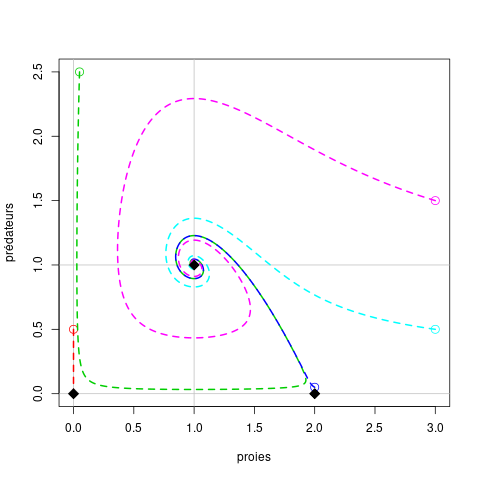
\includegraphics[width=.5\textwidth, trim=0 0 30 60, clip=]{L3bioSU-ProiePredateur-paths}
  $$
  $$
  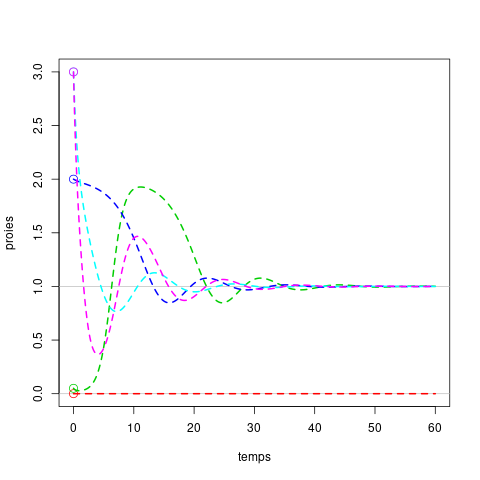
\includegraphics[width=.45\textwidth, trim=0 0 30 60, clip=]{L3bioSU-ProiePredateur-proies}
  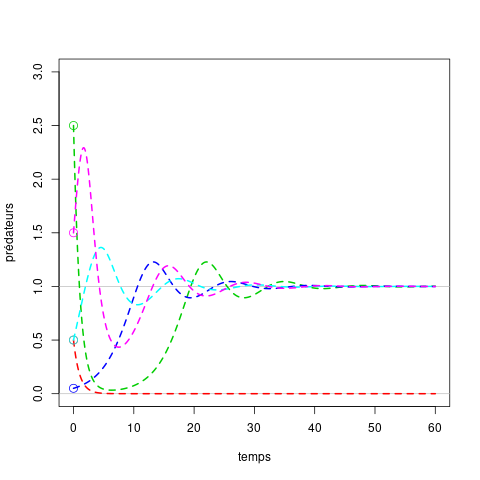
\includegraphics[width=.45\textwidth, trim=0 0 30 60, clip=]{L3bioSU-ProiePredateur-predateurs}
  $$
  }
\end{enumerate}
